\documentclass[12pt]{article}

\usepackage{a4wide} % уменьшает поля
\usepackage[utf8]{inputenc}
\usepackage[russian]{babel} % включает русский язык
\usepackage{graphicx} % позволяет подключить .eps - файлы
\usepackage{amsmath}
\usepackage{amsthm} % теоремы от AMS
\usepackage{amssymb} % для работы с математическими R и проч.
\usepackage{floatrow}
\usepackage{mathrsfs}
\usepackage[section]{placeins}
\usepackage{indentfirst} % абзац после заголовка
\usepackage{misccorr} % точки в заголовках

%\graphicspath{{pics/}}


%\newtheoremstyle{rusdef}
%  {3pt}% measure of space to leave above the theorem. E.g.: 3pt
%  {3pt}% measure of space to leave below the theorem. E.g.: 3pt
%  {\itshape}% name of font to use in the body of the theorem
%  {\parindent}% measure of space to indent
%  {\bfseries}% name of head font
%  {.}%
%  {.5em}%
%  {}


\theoremstyle{rusdef}
\renewcommand\qedsymbol{$\blacksquare$}
\newtheorem{remark}{Замечание}
\newtheorem{theorem}{Теорема}
\newtheorem{definition}{Определение}
\newtheorem{proposition}{Утверждение}

\newcommand*{\hm}[1]{#1\nobreak\discretionary{}{\hbox{$\mathsurround=0pt #1$}}{}}
\newcommand{\scalar}[2]{\left<#1,#2\right>}
\newcommand{\const}{\ensuremath{\operatorname{const}}}
\newcommand{\sgn}{\ensuremath{\operatorname{sgn}}}
\renewcommand{\d}[1]{\ensuremath{\operatorname{d}\!{#1}}}
\newcommand\abs[1]{\left\lvert #1 \right\rvert} % модуль
\newcommand\brackets[1]{\left( #1 \right)} % скобки
\newcommand{\R}{\ensuremath{\mathbb{R}}} % R - мн-во вещественных чисел
\newcommand{\N}{\ensuremath{\mathbb{N}}} % N - мн-во натуральных чисел
\newcommand{\Z}{\ensuremath{\mathbb{Z}}} % Z - мн-во целых чисел
\renewcommand{\C}{\ensuremath{\mathbb{C}}} % C - мн-во комплексных чисел
\newcommand{\E}{\ensuremath{\mathcal{E}}} % E --- эллипсоид
\newcommand{\norm}[1]{\left\lVert #1 \right\rVert} % норма
\DeclareMathOperator*{\thus}{\Rightarrow} % следствие с возможностью использовать limits
\DeclareMathOperator*{\tolim}{\to} % стремление с возможностью использовать limits
\DeclareMathOperator*{\Argmax}{Argmax} % Argmax с возмножностью использовать limits
\DeclareMathOperator{\rank}{rank} % ранг
\DeclareMathOperator{\e}{e} % экспонента

\newcommand{\rpm}{\sbox0{$1$}\sbox2{$\scriptstyle\pm$}
	\raise\dimexpr(\ht1)/2\relax\box2 } % крутой плюс-минус

\begin{document}
	\thispagestyle{empty}
	
	\begin{center}
		\ \vspace{-3cm}
		
		
\includegraphics[width=0.5\textwidth]{msu.eps}\\
		
		{\scshape Московский Государственный Университет имени М.~В.~Ломоносова}\\
		Факультет Вычислительной Математики и Кибернетики\\
		Кафедра Системного Анализа
		\vfill
		
		{\LARGE Анализ системы типа муравейник}
		\vspace{.5cm}
		
	\end{center}
	
	\vspace{1cm}
	
	\begin{flushright}
		\large
		\textit{Студент 515 группы}\\
		В.~С.~Терёшин\\
		\vspace{5mm}
		\textit{Руководитель практики}\\
		д.ф.~-м.н., профессор А. С. Братусь
		
	\end{flushright}
	
	\vfill
	
	\begin{center}
		{\large
			Москва, 2014г.}
	\end{center}
	
	\newpage
	\tableofcontents
	\newpage
	
	\section{Постановка задачи}
	
	Рассматривается динамическая система
	$$
	\left\{
	\begin{aligned}
	\dot{u_1} = u_1 \left( \alpha u_4 + k_1 u_2 + k_2 u_3 - \overline{f} \right), \\
	\dot{u_2} = u_2 \left( \alpha u_4 + k_1 u_3 + k_2 u_1 - \overline{f} \right), \\
	\dot{u_3} = u_3 \left( \alpha u_4 + k_1 u_1 + k_2 u_2 - \overline{f} \right), \\
	\dot{u_4} = u_4 \left( \beta \left( u_1 + u_2 + u_3 \right) - \overline{f} \right).
	\end{aligned}
	\right.
	$$
	при условиях $u_1 + u_2 + u_3 + u_4 = 1$, $\alpha > 0$, $\beta > 0$, $k_1 > 0$, $k_2 > 0$. Введём обозначение $S = u_1 + u_2 + u_3$.
	
	\section{Физический смысл задачи}
	
	Данная система представляет собой описание колонии муравьёв. Королева ($u_4$) обслуживается остальными членами популяции ($u_1$, $u_2$ и $u_3$), которые помогают ей размножаться. В свою очередь, королева колонии способствует размножению других видов муравьёв. Муравьи первого, второго и третьего типов также способствуют размножению друг друга.
	
	\section{Нахождение фитнеса}
	
	Для нахождения фитнеса заметим, что так как $u_1 + u_2 + u_3 + u_4 = 1$, то $\dot{u_1} + \dot{u_2} + \dot{u_3} + \dot{u_4} = 0$. Выпишем уравнение на $\overline{f}$:
	\begin{gather}
	0 = u_1 \left( \alpha u_4 + k_1 u_2 + k_2 u_3 - \overline{f} \right) + \notag \\
	+ u_2 \left( \alpha u_4 + k_1 u_3 + k_2 u_1 - \overline{f} \right) + \notag \\
	+ u_3 \left( \alpha u_4 + k_1 u_1 + k_2 u_2 - \overline{f} \right) + \notag \\
	+ u_4 \left( \beta \left( u_1 + u_2 + u_3 \right) - \overline{f} \right) = \notag \\
	= (\alpha + \beta) u_4 (u_1 + u_2 + u_3) + (k_1 + k_2) (u_1 u_2 + u_1 u_3 + u_2 u_3) - (u_1 + u_2 + u_3 + u_4) \overline{f}. \notag
	\end{gather}
	
	Принимая во внимание то, что $S = u_1 + u_2 + u_3$, а $u_1 + u_2 + u_3 + u_4 = 1$, получим
	\begin{gather}
	0 = (\alpha + \beta) (1 - S) S + (k_1 + k_2) (u_1 u_2 + u_1 u_3 + u_2 u_3) - \overline{f}, \notag \\
	\Rightarrow \overline{f} = (\alpha + \beta) (1 - S) S + (k_1 + k_2) (u_1 u_2 + u_1 u_3 + u_2 u_3). \notag
	\end{gather}
	
	\section{Исследование системы}
	\subsection{Нахождение неподвижных точек}
	
	С помощью символьных вычислений среды \texttt{MATLAB} можно получить неподвижные точки системы:
	\begin{enumerate}
	\item
	$u_1 = 0, \; u_2 = 0, \; u_3 = 0, \; u_4 = a$;
	\item
	$u_1 = 1, \; u_2 = 0, \; u_3 = 0, \; u_4 = 0$;
	\item
	$u_1 = 0, \; u_2 = 1, \; u_3 = 0, \; u_4 = 0$;
	\item
	$u_1 = 0, \; u_2 = 0, \; u_3 = 1, \; u_4 = 0$;
	\item
	$u_1 = \tfrac{1}{3}, \; u_2 = \tfrac{1}{3}, \; u_3 = \tfrac{1}{3}, \; u_4 = 0$;
	\item
	$u_1 = 0, \; u_2 = 0, \; u_3 = \tfrac{\alpha}{\alpha + \beta}, \; u_4 = \tfrac{\beta}{\alpha + \beta}$;
	\item
	$u_1 = 0, \; u_2 = \tfrac{\alpha}{\alpha + \beta}, \; u_3 = 0, \; u_4 = \tfrac{\beta}{\alpha + \beta}$;
	\item
	$u_1 = \tfrac{\alpha}{\alpha + \beta}, \; u_2 = 0, \; u_3 = 0, \; u_4 = \tfrac{\beta}{\alpha + \beta}$;
	\item
	$u_1 = \tfrac{k_1}{k_1 + k_2}, \; u_2 = \tfrac{k_2}{k_1 + k_2}, \; u_3 = 0, \; u_4 = 0$;
	\item
	$u_1 = 0, \; u_2 = \tfrac{k_1}{k_1 + k_2}, \; u_3 = \tfrac{k_2}{k_1 + k_2}, \; u_4 = 0$;
	\item
	$u_1 = \tfrac{k_2}{k_1 + k_2}, \; u_2 = \tfrac{k_1}{k_1 + k_2}, \; u_3 = 0, \; u_4 = 0$;
	\item
	$u_1 = \tfrac{\alpha k_1}{(\alpha + \beta)(k_1 + k_2) - k_1 k_2}, \; u_2 = \tfrac{\alpha k_2}{(\alpha + \beta)(k_1 + k_2) - k_1 k_2}, \; u_3 = 0, \; u_4 = \tfrac{(k_1 + k_2) \beta - k_1 k_2}{(\alpha + \beta)(k_1 + k_2) - k_1 k_2}$;
	\item
	$u_1 = 0, \; u_2 = \tfrac{\alpha k_1}{(\alpha + \beta)(k_1 + k_2) - k_1 k_2}, \; u_3 = \tfrac{\alpha k_2}{(\alpha + \beta)(k_1 + k_2) - k_1 k_2}, \; u_4 = \tfrac{(k_1 + k_2) \beta - k_1 k_2}{(\alpha + \beta)(k_1 + k_2) - k_1 k_2}$;
	\item
	$u_1 = \tfrac{\alpha k_2}{(\alpha + \beta)(k_1 + k_2) - k_1 k_2}, \; u_2 = 0, \; u_3 = \tfrac{\alpha k_1}{(\alpha + \beta)(k_1 + k_2) - k_1 k_2}, \; u_4 = \tfrac{(k_1 + k_2) \beta - k_1 k_2}{(\alpha + \beta)(k_1 + k_2) - k_1 k_2}$;
	\item
	$u_1 = \tfrac{\alpha}{3(\alpha + \beta) - k_1 - k_2}, \; u_2 = \tfrac{\alpha}{3(\alpha + \beta) - k_1 - k_2}, \; u_3 = \tfrac{\alpha}{3(\alpha + \beta) - k_1 - k_2}, \; u_4 = \tfrac{3\beta - k_1 - k_2}{3(\alpha + \beta) - k_1 - k_2}$;
	\end{enumerate}
	
	\subsection{Нахождение якобиана системы}
	
	Якобиан данной системы равен:
	\begin{gather}
	J(u_1, u_2, u_3, u_4) = \left[
	\begin{array}{cccc}
	\frac{df_1}{du_1} & \frac{df_1}{du_2} & \frac{df_1}{du_3} & \frac{df_1}{du_4} \\[0.5em]
	\frac{df_2}{du_1} & \frac{df_2}{du_2} & \frac{df_2}{du_3} & \frac{df_2}{du_4} \\[0.5em]
	\frac{df_3}{du_1} & \frac{df_3}{du_2} & \frac{df_3}{du_3} & \frac{df_3}{du_4} \\[0.5em]
	\frac{df_4}{du_1} & \frac{df_4}{du_2} & \frac{df_4}{du_3} & \frac{df_4}{du_4}
	\end{array} \right] \notag
%	\right] = \notag \\
%	\left(\begin{array}{cccc} \alpha\, u_{4} + k_{1}\, u_{2} + k_{2}\, u_{3} + u_{1}\, \left(\left(\alpha + \beta\right)\, \left(u_{1} + u_{2} + u_{3}\right) + \left(\alpha + \beta\right)\, \left(u_{1} + u_{2} + u_{3} - 1\right) - \left(k_{1} + k_{2}\right)\, \left(u_{2} + u_{3}\right)\right) - \left(k_{1} + k_{2}\right)\, \left(u_{1}\, u_{2} + u_{1}\, u_{3} + u_{2}\, u_{3}\right) + \left(\alpha + \beta\right)\, \left(u_{1} + u_{2} + u_{3}\right)\, \left(u_{1} + u_{2} + u_{3} - 1\right) & u_{1}\, \left(k_{1} + \left(\alpha + \beta\right)\, \left(u_{1} + u_{2} + u_{3}\right) + \left(\alpha + \beta\right)\, \left(u_{1} + u_{2} + u_{3} - 1\right) - \left(k_{1} + k_{2}\right)\, \left(u_{1} + u_{3}\right)\right) & u_{1}\, \left(k_{2} + \left(\alpha + \beta\right)\, \left(u_{1} + u_{2} + u_{3}\right) + \left(\alpha + \beta\right)\, \left(u_{1} + u_{2} + u_{3} - 1\right) - \left(k_{1} + k_{2}\right)\, \left(u_{1} + u_{2}\right)\right) & \alpha\, u_{1}\\ u_{2}\, \left(k_{2} + \left(\alpha + \beta\right)\, \left(u_{1} + u_{2} + u_{3}\right) + \left(\alpha + \beta\right)\, \left(u_{1} + u_{2} + u_{3} - 1\right) - \left(k_{1} + k_{2}\right)\, \left(u_{2} + u_{3}\right)\right) & \alpha\, u_{4} + k_{2}\, u_{1} + k_{1}\, u_{3} + u_{2}\, \left(\left(\alpha + \beta\right)\, \left(u_{1} + u_{2} + u_{3}\right) + \left(\alpha + \beta\right)\, \left(u_{1} + u_{2} + u_{3} - 1\right) - \left(k_{1} + k_{2}\right)\, \left(u_{1} + u_{3}\right)\right) - \left(k_{1} + k_{2}\right)\, \left(u_{1}\, u_{2} + u_{1}\, u_{3} + u_{2}\, u_{3}\right) + \left(\alpha + \beta\right)\, \left(u_{1} + u_{2} + u_{3}\right)\, \left(u_{1} + u_{2} + u_{3} - 1\right) & u_{2}\, \left(k_{1} + \left(\alpha + \beta\right)\, \left(u_{1} + u_{2} + u_{3}\right) + \left(\alpha + \beta\right)\, \left(u_{1} + u_{2} + u_{3} - 1\right) - \left(k_{1} + k_{2}\right)\, \left(u_{1} + u_{2}\right)\right) & \alpha\, u_{2}\\ u_{3}\, \left(k_{1} + \left(\alpha + \beta\right)\, \left(u_{1} + u_{2} + u_{3}\right) + \left(\alpha + \beta\right)\, \left(u_{1} + u_{2} + u_{3} - 1\right) - \left(k_{1} + k_{2}\right)\, \left(u_{2} + u_{3}\right)\right) & u_{3}\, \left(k_{2} + \left(\alpha + \beta\right)\, \left(u_{1} + u_{2} + u_{3}\right) + \left(\alpha + \beta\right)\, \left(u_{1} + u_{2} + u_{3} - 1\right) - \left(k_{1} + k_{2}\right)\, \left(u_{1} + u_{3}\right)\right) & \alpha\, u_{4} + k_{1}\, u_{1} + k_{2}\, u_{2} + u_{3}\, \left(\left(\alpha + \beta\right)\, \left(u_{1} + u_{2} + u_{3}\right) + \left(\alpha + \beta\right)\, \left(u_{1} + u_{2} + u_{3} - 1\right) - \left(k_{1} + k_{2}\right)\, \left(u_{1} + u_{2}\right)\right) - \left(k_{1} + k_{2}\right)\, \left(u_{1}\, u_{2} + u_{1}\, u_{3} + u_{2}\, u_{3}\right) + \left(\alpha + \beta\right)\, \left(u_{1} + u_{2} + u_{3}\right)\, \left(u_{1} + u_{2} + u_{3} - 1\right) & \alpha\, u_{3}\\ u_{4}\, \left(\beta + \left(\alpha + \beta\right)\, \left(u_{1} + u_{2} + u_{3}\right) + \left(\alpha + \beta\right)\, \left(u_{1} + u_{2} + u_{3} - 1\right) - \left(k_{1} + k_{2}\right)\, \left(u_{2} + u_{3}\right)\right) & u_{4}\, \left(\beta + \left(\alpha + \beta\right)\, \left(u_{1} + u_{2} + u_{3}\right) + \left(\alpha + \beta\right)\, \left(u_{1} + u_{2} + u_{3} - 1\right) - \left(k_{1} + k_{2}\right)\, \left(u_{1} + u_{3}\right)\right) & u_{4}\, \left(\beta + \left(\alpha + \beta\right)\, \left(u_{1} + u_{2} + u_{3}\right) + \left(\alpha + \beta\right)\, \left(u_{1} + u_{2} + u_{3} - 1\right) - \left(k_{1} + k_{2}\right)\, \left(u_{1} + u_{2}\right)\right) & \beta\, \left(u_{1} + u_{2} + u_{3}\right) - \left(k_{1} + k_{2}\right)\, \left(u_{1}\, u_{2} + u_{1}\, u_{3} + u_{2}\, u_{3}\right) + \left(\alpha + \beta\right)\, \left(u_{1} + u_{2} + u_{3}\right)\, \left(u_{1} + u_{2} + u_{3} - 1\right) \end{array}\right)
	%\left[
	%\begin{array}{cccc}
	%\alpha u_4 + k_1 u_2 + k_2 u_3 - \overline{f} & k_1 u_1 & k_2 u_1 & \alpha u_1 \\
	%k_2 u_2 & \alpha u_4 + k_1 u_3 + k_2 u_1 - \overline{f} & k_1 u_2 & \alpha u_2 \\
	%k_1 u_3 & k_2 u_3 & \alpha u_4 + k_1 u_1 + k_2 u_2 - \overline{f} & \alpha u_3 \\
	%\beta u_4 & \beta u_4 & \beta u_4 & \beta \left( u_1 + u_2 + u_3 \right) - \overline{f}
	%\end{array}
	%\right] \notag
	\end{gather}
	
	К сожалению, выписать в полном виде якобиан данной системы на данном формате бумаги не представляется возможным. Он был вычислен с помощью символьных вычислений среды \texttt{MATLAB}, как и собственные числа далее.
	
	\subsection{Исследование неподвижных точек на устойчивость}
	
	Изолированные неподвижные точки можно проверить на устойчивость, воспользовавшись следующей теоремой:
	
	\begin{definition}[Гиперболическое положение равновесия]
	Положение равновесия динамической системы называется гиперболическим, если не существует собственных значений якобиана системы в этой точке, расположенных на мнимой оси.
	\end{definition}
	
	\begin{theorem}[Ляпунов, Пуанкаре]
	Пусть $u^*$ --- гиперболическое положение равновесия системы. Пусть $n_+$, $n_-$ --- число собственных значений $J(u^*)$ с положительной и отрицательной вещественной частью соответственно. Тогда, если $n_+ = 0$, то положение равновесия ассимптотически устойчиво, а если $n_+ > 0$, то неустойчиво.
	\end{theorem}
	
	\subsubsection{Исследование положения равновесия 1}
	
	Чтобы удовлетворять условию задачи, необходимо чтобы $a = 1$. В этом случае $\overline{f} = 0$.
	
	\begin{gather}
	J(0, 0, 0, 1) = \left[
	\begin{array}{cccc}
	\alpha & 0 & 0 & 0 \\[0.5em]
	0 & \alpha & 0 & 0 \\[0.5em]
	0 & 0 & \alpha & 0 \\[0.5em]
	\alpha & \alpha & \alpha & 0
	\end{array}
	\right] = \notag
	\end{gather}

	Собственными значениями данной матрицы являются числа:
	\begin{enumerate}
		\item
		$\lambda_1 = 0$;
		\item
		$\lambda_2 = \alpha$;
		\item
		$\lambda_3 = \alpha$;
		\item
		$\lambda_4 = \alpha$;
	\end{enumerate}
	
	Из собственных значений невозможно установить устойчивость неподвижной точки и необходимо провести дополнительное исследование.

	\subsubsection{Исследование положений равновесия 2--4}
	
	В силу симметрии системы можно исследовать любое из этих положений равновесия: остальные будут обладать такими же свойствами. Рассмотрим, например, положении равновесия $(1, 0, 0, 0)$. В этом случае $\overline{f} = 0$.
	
	\begin{gather}
	J(1, 0, 0, 0) = \left[
\begin{array}{cccc} \alpha + \beta & \alpha + \beta - k_2 & \alpha + \beta - k_1 & \alpha\\ 0 & k_2 & 0 & 0\\ 0 & 0 & k_1 & 0\\ 0 & 0 & 0 & \beta \end{array}	%\begin{array}{cccc}
	%0 & k_1 & k_2 & \alpha \\[0.5em]
	%0 & k_2 & 0 & 0 \\[0.5em]
	%0 & 0 & k_1 & 0 \\[0.5em]
	%0 & 0 & 0 & \beta
	%\end{array}
	\right] = \notag
	\end{gather}
	
		
		Собственными значениями данной матрицы являются числа:
		\begin{enumerate}
			\item
			$\lambda_1 = \beta$;
			\item
			$\lambda_2 = k_1$;
			\item
			$\lambda_3 = k_2$;
			\item
			$\lambda_4 = \alpha+\beta$;
		\end{enumerate}
		
		Из собственных значений и теоремы видно, что данная точка является неустойчивой.
	
	\subsubsection{Исследование положения равновесия 5}
	
	В этом случае $\overline{f} = \tfrac{k_1 + k_2}{3}$, а
	\begin{gather}
	J\left(\frac{1}{3}, \frac{1}{3}, \frac{1}{3}, 0\right) = \left[
\begin{array}{cccc} \frac{\alpha}{3} + \frac{\beta}{3} - \frac{2\, k_{1}}{9} - \frac{2\, k_{2}}{9} & \frac{\alpha}{3} + \frac{\beta}{3} + \frac{k_{1}}{9} - \frac{2\, k_{2}}{9} & \frac{\alpha}{3} + \frac{\beta}{3} - \frac{2\, k_{1}}{9} + \frac{k_{2}}{9} & \frac{\alpha}{3}\\ \frac{\alpha}{3} + \frac{\beta}{3} - \frac{2\, k_{1}}{9} + \frac{k_{2}}{9} & \frac{\alpha}{3} + \frac{\beta}{3} - \frac{2\, k_{1}}{9} - \frac{2\, k_{2}}{9} & \frac{\alpha}{3} + \frac{\beta}{3} + \frac{k_{1}}{9} - \frac{2\, k_{2}}{9} & \frac{\alpha}{3}\\ \frac{\alpha}{3} + \frac{\beta}{3} + \frac{k_{1}}{9} - \frac{2\, k_{2}}{9} & \frac{\alpha}{3} + \frac{\beta}{3} - \frac{2\, k_{1}}{9} + \frac{k_{2}}{9} & \frac{\alpha}{3} + \frac{\beta}{3} - \frac{2\, k_{1}}{9} - \frac{2\, k_{2}}{9} & \frac{\alpha}{3}\\ 0 & 0 & 0 & \beta - \frac{k_{1}}{3} - \frac{k_{2}}{3} \end{array}
%	\begin{array}{cccc}
%	0 & k_1/3 & k_2/3 & \alpha/3 \\[0.5em]
%	k_2/3 & 0 & k_1/3 & \alpha/3 \\[0.5em]
%	k_1/3 & k_2/3 & 0 & \alpha/3 \\[0.5em]
%	0 & 0 & 0 & \beta - \frac{k_1 + k_2}{3}
%	\end{array}
	\right]. \notag
	\end{gather}
	
	Собственными значениями данной матрицы являются числа:
	\begin{enumerate}
	\item
	$\lambda_1 = \beta - \frac{k_1 + k_2}{3}$;
	\item
	$\lambda_2 = \alpha + \beta - \frac{k_1 + k_2}{3}$;
	\item
	$\lambda_3 = -\frac{k_1+k_2}{6} - \frac{\sqrt{3}(k_1-k2)}{6}i$;
	\item
	$\lambda_4 = -\frac{k_1+k_2}{6} + \frac{\sqrt{3}(k_1-k2)}{6}i$;
	\end{enumerate}
	
	Из собственных значений и теоремы видно, что данная точка является ассимптотический устойчивой, если $\alpha + \beta < \frac{k_1+k_2}{3}$, неустойчивой, если $\alpha + \beta > \frac{k_1+k_2}{3}$, а в случае $\alpha + \beta = \frac{k_1+k_2}{3}$ необходимо дополнительное исследование.
	
	\subsubsection{Исследование положений равновесия 6--8}
	
	В силу симметрии будем исследовать положение равновесия $\left( \frac{\alpha}{\alpha+\beta}, 0, 0, \frac{\beta}{\alpha+\beta} \right)$. В этом случае $\overline{f} = \frac{\alpha\beta}{\alpha+\beta}$.

	\begin{gather}
	J\left( \frac{\alpha}{\alpha+\beta}, 0, 0, \frac{\beta}{\alpha+\beta} \right) = \left[
\begin{array}{cccc} \frac{\alpha\, \left(\alpha - \beta\right)}{\alpha + \beta} & -\frac{\alpha\, \left( - {\alpha}^2 + k_{2}\, \alpha + {\beta}^2 - 1\, k_{1}\, \beta\right)}{{\left(\alpha + \beta\right)}^2} & -\frac{\alpha\, \left( - {\alpha}^2 + k_{1}\, \alpha + {\beta}^2 - 1\, k_{2}\, \beta\right)}{{\left(\alpha + \beta\right)}^2} & \frac{{\alpha}^2}{\alpha + \beta}\\ 0 & \frac{\alpha\, k_{2}}{\alpha + \beta} & 0 & 0\\ 0 & 0 & \frac{\alpha\, k_{1}}{\alpha + \beta} & 0\\ \frac{\alpha\, \beta}{\alpha + \beta} & \frac{\alpha\, \beta\, \left(\alpha + \beta - k_{1} - k_{2}\right)}{{\left(\alpha + \beta\right)}^2} & \frac{\alpha\, \beta\, \left(\alpha + \beta - k_{1} - k_{2}\right)}{{\left(\alpha + \beta\right)}^2} & 0 \end{array}
%	\begin{array}{cccc}
%	0 & \frac{\alpha k_1}{\alpha + \beta} & \frac{\alpha k_2}{\alpha + \beta} & \frac{\alpha^2}{\alpha+\beta} \\[0.5em]
%	0 & \frac{\alpha k_2}{\alpha + \beta} & 0 & 0 \\[0.5em]
%	0 & 0 & \frac{\alpha k_1}{\alpha + \beta} & 0 \\[0.5em]
%	\frac{\beta^2}{\alpha+\beta} & \frac{\beta^2}{\alpha+\beta} & \frac{\beta^2}{\alpha+\beta} & 0
%	\end{array}
	\right]. \notag
	\end{gather}
	
	Собственными значениями данной матрицы являются числа:
	\begin{enumerate}
		\item
		$\lambda_1 = \frac{\alpha^2}{\alpha + \beta}$;
		\item
		$\lambda_2 = -\frac{\alpha \beta}{\alpha + \beta}$;
		\item
		$\lambda_3 = \frac{\alpha k_1}{\alpha + \beta}$;
		\item
		$\lambda_4 = \frac{\alpha k_2}{\alpha + \beta}$;
	\end{enumerate}
	
	Из собственных значений и теоремы видно, что данная точка является неустойчивой, как и другие в этой группе.
	
	\subsubsection{Исследование положений равновесия 9--11}
	
	Будем исследовать положение равновесия 	$\left( \tfrac{k_1}{k_1 + k_2}, \tfrac{k_2}{k_1 + k_2}, 0, 0 \right)$. В этом случае $\overline{f} \hm= \frac{k_1 k_2}{k_1 + k_2}$.
	
	\begin{gather}
	J\left(  \tfrac{k_1}{k_1 + k_2}, \tfrac{k_2}{k_1 + k_2}, 0, 0 \right) = \left[
\begin{array}{cccc} \frac{k_{1}\, \left(\alpha + \beta - k_{2}\right)}{k_{1} + k_{2}} & \frac{k_{1}\, \left(\alpha + \beta\right)}{k_{1} + k_{2}} & \frac{k_{1}\, \left(\alpha + \beta - k_{1}\right)}{k_{1} + k_{2}} & \frac{\alpha\, k_{1}}{k_{1} + k_{2}}\\ \frac{k_{2}\, \left(\alpha + \beta\right)}{k_{1} + k_{2}} & \frac{k_{2}\, \left(\alpha + \beta - k_{1}\right)}{k_{1} + k_{2}} & \frac{k_{2}\, \left(\alpha + \beta - k_{2}\right)}{k_{1} + k_{2}} & \frac{\alpha\, k_{2}}{k_{1} + k_{2}}\\ 0 & 0 & \frac{{k_{1}}^2 - k_{1}\, k_{2} + {k_{2}}^2}{k_{1} + k_{2}} & 0\\ 0 & 0 & 0 & \frac{\beta\, k_{1} + \beta\, k_{2} - k_{1}\, k_{2}}{k_{1} + k_{2}} \end{array}
%	\begin{array}{cccc}
%	0 & \frac{k_1^2}{k_1+k_2} & \frac{k_1 k_2}{k_1+k_2} & \frac{\alpha k_1}{k_1+k_2} \\[0.5em]
%	\frac{k2^2}{k_1+k_2} & 0 & \frac{k_1 k_2}{k_1+k_2} & \frac{\alpha k_2}{k_1+k_2} \\[0.5em]
%	0 & 0 & \frac{k_1^2 - k_1k_2 + k_2^2}{k_1+k_2} & 0 \\[0.5em]
%	0 & 0 & 0 & \beta - \frac{k_1 k_2}{k_1+k_2}
%	\end{array}
	\right]. \notag
	\end{gather}
	
	Собственными значениями данной матрицы являются числа:
	\begin{enumerate}
		\item
		$\lambda_1 = \frac{k_1^2 - k_1 k_2 + k_2^2}{k_1+k_2}$;
		\item
		$\lambda_2 = \alpha + \beta - \frac{k_1 k_2}{k_1+k_2}$;
		\item
		$\lambda_3 = \beta - \frac{k_1 k_2}{k_1+k_2}$;
		\item
		$\lambda_4 = -\frac{k_1 k_2}{k_1+k_2}$;
	\end{enumerate}
	
	Рассмотрим числитель $\lambda_1$:
	\begin{gather}
	k_1^2 - k_1 k_2 + k_2^2 = (k_1 - k_2)^2 + k_1 k_2 > 0. \notag
	\end{gather}
	
	Из собственных значений и теоремы видно, что данная точка является неустойчивой, как и другие в этой группе, если $\beta \neq \tfrac{k_1k_2}{k_1+k_2}$ и $\alpha + \beta \neq \tfrac{k_1k_2}{k_1+k_2}$.
	
	\subsubsection{Исследование положений равновесия 12--14}

	Данные положения равновесия существуют при $k_1 k_2 < \beta(k_1 + k_2)$.

	Будем исследовать положение равновесия 
	$$
	\left( \tfrac{\alpha k_1}{(\alpha + \beta)(k_1 + k_2) - k_1 k_2}, \tfrac{\alpha k_2}{(\alpha + \beta)(k_1 + k_2) - k_1 k_2}, 0, \tfrac{(k_1 + k_2) \beta - k_1 k_2}{(\alpha + \beta)(k_1 + k_2) - k_1 k_2} \right).
	$$

	К сожеланию, якобиан и его собственные значения в этих точках имеют слишком громоздкий вид, поэтому мы его приводить не будем. Заметим лишь, что с помощью символьных вычислений среды \texttt{MATLAB} удалось установить, что эти точки почти всегда являются неустойчивыми положениями равновесия (существуют противоположные по знаку вещественные собственные значения).
	
	\subsubsection{Исследование положений равновесия 15}
	
	Данное положение равновесия существует при $k_1 + k_2 < 3\beta$.

	Будем исследовать положение равновесия 
	$$
	\left( \tfrac{\alpha}{3(\alpha + \beta) - k_1 - k_2}, \tfrac{\alpha}{3(\alpha + \beta) - k_1 - k_2}, \tfrac{\alpha}{3(\alpha + \beta) - k_1 - k_2}, \tfrac{3\beta - k_1 - k_2}{3(\alpha + \beta) - k_1 - k_2} \right).
	$$

	\begin{gather}
	J\left( \tfrac{\alpha}{3(\alpha + \beta) - k_1 - k_2}, \tfrac{\alpha}{3(\alpha + \beta) - k_1 - k_2}, \tfrac{\alpha}{3(\alpha + \beta) - k_1 - k_2}, \tfrac{3\beta - k_1 - k_2}{3(\alpha + \beta) - k_1 - k_2} \right) = \notag \\
	= \left[
\begin{array}{cccc} \frac{\alpha\, \left(\alpha - \beta\right)}{3\, \alpha + 3\, \beta - k_{1} - k_{2}} & \frac{\alpha\, \left(\alpha - \beta + k_{1}\right)}{3\, \alpha + 3\, \beta - k_{1} - k_{2}} & \frac{\alpha\, \left(\alpha - \beta + k_{2}\right)}{3\, \alpha + 3\, \beta - k_{1} - k_{2}} & \frac{{\alpha}^2}{3\, \alpha + 3\, \beta - k_{1} - k_{2}}\\ \frac{\alpha\, \left(\alpha - \beta + k_{2}\right)}{3\, \alpha + 3\, \beta - k_{1} - k_{2}} & \frac{\alpha\, \left(\alpha - \beta\right)}{3\, \alpha + 3\, \beta - k_{1} - k_{2}} & \frac{\alpha\, \left(\alpha - \beta + k_{1}\right)}{3\, \alpha + 3\, \beta - k_{1} - k_{2}} & \frac{{\alpha}^2}{3\, \alpha + 3\, \beta - k_{1} - k_{2}}\\ \frac{\alpha\, \left(\alpha - \beta + k_{1}\right)}{3\, \alpha + 3\, \beta - k_{1} - k_{2}} & \frac{\alpha\, \left(\alpha - \beta + k_{2}\right)}{3\, \alpha + 3\, \beta - k_{1} - k_{2}} & \frac{\alpha\, \left(\alpha - \beta\right)}{3\, \alpha + 3\, \beta - k_{1} - k_{2}} & \frac{{\alpha}^2}{3\, \alpha + 3\, \beta - k_{1} - k_{2}}\\ -\frac{\alpha\, \left(k_{1} - 3\, \beta + k_{2}\right)}{3\, \alpha + 3\, \beta - k_{1} - k_{2}} & -\frac{\alpha\, \left(k_{1} - 3\, \beta + k_{2}\right)}{3\, \alpha + 3\, \beta - k_{1} - k_{2}} & -\frac{\alpha\, \left(k_{1} - 3\, \beta + k_{2}\right)}{3\, \alpha + 3\, \beta - k_{1} - k_{2}} & 0 \end{array}
	\right]. \notag
	\end{gather}

	Собственными значениями данной матрицы являются числа:
	\begin{enumerate}
		\item
		$\lambda_1 = \frac{\alpha(k_1 + k_2 - 3\beta)}{3(\alpha + \beta) - k_1 - k_2}$;
		\item
		$\lambda_2 = -\frac{3\alpha^2}{3(\alpha + \beta) - k_1 - k_2}$;
		\item
		$\lambda_3 = \frac{1}{2(3(\alpha + \beta) - k_1 - k_2)} \left( -\alpha(k_1 + k_2) - \sqrt{3} (k_1 - k_2)i \right)$;
		\item
		$\lambda_4 = \frac{1}{2(3(\alpha + \beta) - k_1 - k_2)} \left( -\alpha(k_1 + k_2) + \sqrt{3} (k_1 - k_2)i \right)$;
	\end{enumerate}
	
	%В число собственных значений якобиана в этой точке входит $\lambda = \tfrac{3\alpha^2}{3(\alpha + \beta) - k_1 - k_2}$, которое является положительным. Вещественные части других собственных значений не обращаются в $0$ при данных ограничениях на параметры. Таким образом, данная точка не является устойчивой при любых допустимых параметрах.

	Из собственных значений, полученных с помощью \texttt{MATLAB}, видно, что данная неподвижная точка является устойчивой, когда существует, то есть когда $k_1 + k_2 < 3\beta$.

	\section{Примеры}
	
	Примеры динамики системы с разными параметрами были построены в среде \texttt{MATLAB}.
	\subsection{Пример 1: случай 3}

	В данном примере $\alpha = 0.1, \beta = 0.5, k_1 = 0.5, k_2 = 1$:
	
	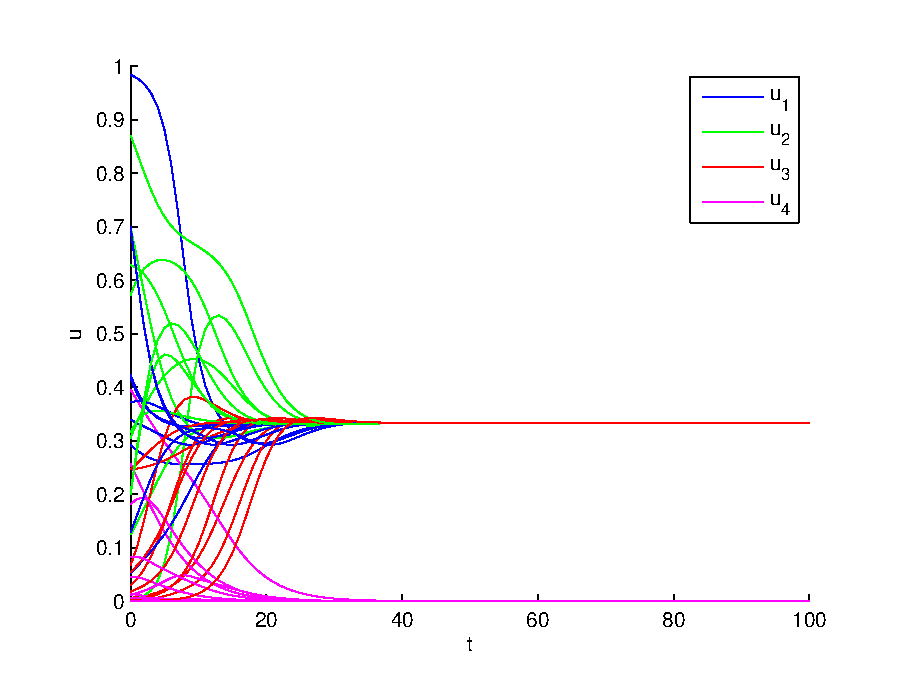
\includegraphics{pics/3.eps}

	\subsection{Пример 2: случай 15}
	
	В данном примере $\alpha = 0.1, \beta = 0.8, k_1 = 0.5, k_2 = 1$:
	
	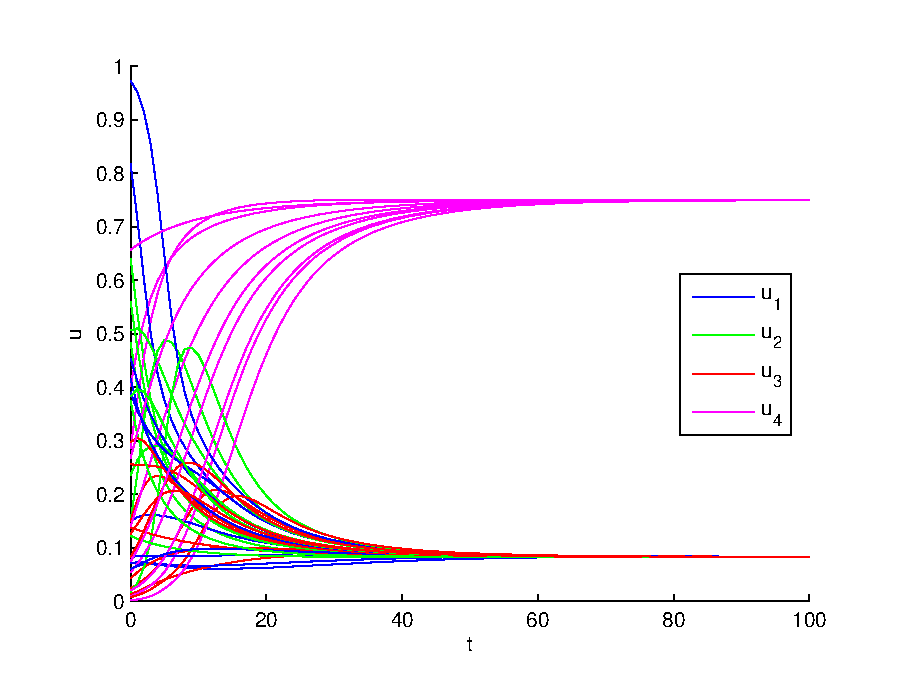
\includegraphics{pics/15.eps}

\end{document}